% Options for packages loaded elsewhere
\PassOptionsToPackage{unicode}{hyperref}
\PassOptionsToPackage{hyphens}{url}
\PassOptionsToPackage{dvipsnames,svgnames,x11names}{xcolor}
%
\documentclass[
  11pt,
]{article}
\usepackage{amsmath,amssymb}
\usepackage{iftex}
\ifPDFTeX
  \usepackage[T1]{fontenc}
  \usepackage[utf8]{inputenc}
  \usepackage{textcomp} % provide euro and other symbols
\else % if luatex or xetex
  \usepackage{unicode-math} % this also loads fontspec
  \defaultfontfeatures{Scale=MatchLowercase}
  \defaultfontfeatures[\rmfamily]{Ligatures=TeX,Scale=1}
\fi
\usepackage{lmodern}
\ifPDFTeX\else
  % xetex/luatex font selection
\fi
% Use upquote if available, for straight quotes in verbatim environments
\IfFileExists{upquote.sty}{\usepackage{upquote}}{}
\IfFileExists{microtype.sty}{% use microtype if available
  \usepackage[]{microtype}
  \UseMicrotypeSet[protrusion]{basicmath} % disable protrusion for tt fonts
}{}
\makeatletter
\@ifundefined{KOMAClassName}{% if non-KOMA class
  \IfFileExists{parskip.sty}{%
    \usepackage{parskip}
  }{% else
    \setlength{\parindent}{0pt}
    \setlength{\parskip}{6pt plus 2pt minus 1pt}}
}{% if KOMA class
  \KOMAoptions{parskip=half}}
\makeatother
\usepackage{xcolor}
\usepackage[margin=2.5cm]{geometry}
\usepackage{longtable,booktabs,array}
\usepackage{calc} % for calculating minipage widths
% Correct order of tables after \paragraph or \subparagraph
\usepackage{etoolbox}
\makeatletter
\patchcmd\longtable{\par}{\if@noskipsec\mbox{}\fi\par}{}{}
\makeatother
% Allow footnotes in longtable head/foot
\IfFileExists{footnotehyper.sty}{\usepackage{footnotehyper}}{\usepackage{footnote}}
\makesavenoteenv{longtable}
\usepackage{graphicx}
\makeatletter
\def\maxwidth{\ifdim\Gin@nat@width>\linewidth\linewidth\else\Gin@nat@width\fi}
\def\maxheight{\ifdim\Gin@nat@height>\textheight\textheight\else\Gin@nat@height\fi}
\makeatother
% Scale images if necessary, so that they will not overflow the page
% margins by default, and it is still possible to overwrite the defaults
% using explicit options in \includegraphics[width, height, ...]{}
\setkeys{Gin}{width=\maxwidth,height=\maxheight,keepaspectratio}
% Set default figure placement to htbp
\makeatletter
\def\fps@figure{htbp}
\makeatother
\setlength{\emergencystretch}{3em} % prevent overfull lines
\providecommand{\tightlist}{%
  \setlength{\itemsep}{0pt}\setlength{\parskip}{0pt}}
\setcounter{secnumdepth}{-\maxdimen} % remove section numbering
\ifLuaTeX
\usepackage[bidi=basic]{babel}
\else
\usepackage[bidi=default]{babel}
\fi
\babelprovide[main,import]{brazilian}
% get rid of language-specific shorthands (see #6817):
\let\LanguageShortHands\languageshorthands
\def\languageshorthands#1{}
% Caracteres Unicode usados no texto (permite compilar com pdflatex; xelatex/lualatex não precisam)
\usepackage{iftex}
\ifPDFTeX
  \usepackage{newunicodechar}
  \newunicodechar{α}{\ensuremath{\alpha}}
  \newunicodechar{λ}{\ensuremath{\lambda}}
  \newunicodechar{↔}{\ensuremath{\leftrightarrow}}
  \newunicodechar{∈}{\ensuremath{\in}}
  \newunicodechar{−}{\ensuremath{-}}
  \newunicodechar{≈}{\ensuremath{\approx}}
  \newunicodechar{≥}{\ensuremath{\geq}}
  \newunicodechar{→}{\ensuremath{\rightarrow}}
  \newunicodechar{×}{\ensuremath{\times}}
  \newunicodechar{·}{\ensuremath{\cdot}}
\fi
\usepackage{float}
\let\origfigure\figure
\let\endorigfigure\endfigure
\renewenvironment{figure}[1][2] {\origfigure[H]} {\endorigfigure}
\ifLuaTeX
  \usepackage{selnolig}  % disable illegal ligatures
\fi
\IfFileExists{bookmark.sty}{\usepackage{bookmark}}{\usepackage{hyperref}}
\IfFileExists{xurl.sty}{\usepackage{xurl}}{} % add URL line breaks if available
\urlstyle{same}
\hypersetup{
  pdftitle={Plataformas de entrega e internações de motociclistas no SUS: carga, custo público e um desenho causal pré-registrado},
  pdfauthor={{[}NOMES DOS AUTORES{]} --- Universidade Federal do Paraná (UFPR)},
  pdflang={pt-BR},
  colorlinks=true,
  linkcolor={Maroon},
  filecolor={Maroon},
  citecolor={Blue},
  urlcolor={Blue},
  pdfcreator={LaTeX via pandoc}}

\title{Plataformas de entrega e internações de motociclistas no SUS:
carga, custo público e um desenho causal pré-registrado}
\usepackage{etoolbox}
\makeatletter
\providecommand{\subtitle}[1]{% add subtitle to \maketitle
  \apptocmd{\@title}{\par {\large #1 \par}}{}{}
}
\makeatother
\subtitle{Versão prévia --- resultados descritivos, construção do
tratamento e plano de identificação}
\author{{[}NOMES DOS AUTORES{]} --- Universidade Federal do Paraná
(UFPR)}
\date{13 de outubro de 2026}

\begin{document}
\maketitle

\textbf{Resumo.} \emph{Problema:} a expansão das plataformas de entrega
com remuneração por corrida coincide com o crescimento das internações
de motociclistas no Sistema Único de Saúde (SUS), mas nenhuma base
administrativa pública liga uma internação ao trabalho por plataforma, e
o debate público trata só do vínculo empregatício, não de quem paga a
conta hospitalar. \emph{Objetivo:} medir a carga e o custo público das
internações de motociclistas, documentar a invisibilidade ocupacional
desses casos nos registros oficiais e construir --- antes de olhar o
desfecho --- um tratamento municipal datado que permita estimar o efeito
causal da chegada do entregador por aplicativo. \emph{Métodos:} painel
município × mês (2015--2025) montado a partir dos microdados do SIH/SUS
(3.563 de 3.564 competências; 433.033 linhas em 5.517 municípios), frota
municipal do Senatran, benefícios do INSS, PNAD Contínua e relatórios da
Prosus. O tratamento é a quebra estrutural nas aberturas de MEI com CNAE
5320-2/02, detectada por uma regra de teste de Poisson cujos
hiperparâmetros foram calibrados por busca em grade contra um placebo
pré-plataforma e contra datas externas (Wayback Machine), nunca contra
internações. O plano de análise (diferenças em diferenças com adoção
escalonada, Callaway \& Sant'Anna) foi registrado no OSF antes de
qualquer cruzamento tratamento × desfecho. \emph{Resultados:} foram
965.714 internações de motociclistas em 2016--2023, das quais 62 (uma em
15.576) registram nexo ocupacional; o SUS pagou R\$ 288 milhões com
essas internações em 2025, enquanto o resultado operacional do iFood no
mesmo ano foi de R\$ 1,8 bilhão. A regra de quebra data 640 municípios
de 20 a 100 mil habitantes entre 2017 e 2025, com falso positivo de
0,7\% a 3,8\% no placebo; 478 entram na janela balanceada de estimação.
\emph{Conclusão:} a carga é grande, crescente e invisível como acidente
de trabalho; o desenho causal é viável e está travado por pré-registro.
Esta versão entrega a parte descritiva e a construção do tratamento; a
estimação causal é a etapa seguinte, já especificada.

\textbf{Palavras-chave:} plataformas digitais; entregadores; acidentes
de motocicleta; SIH/SUS; diferenças em diferenças; pré-registro.

\hypertarget{introduuxe7uxe3o}{%
\section{1. Introdução}\label{introduuxe7uxe3o}}

O Brasil tem hoje cerca de 405 mil motociclistas cuja ocupação principal
é mediada por plataforma digital, quase o dobro dos 211 mil de 2022
(PNAD Contínua, microdado, cálculo próprio). Esse contingente trabalha
com 85\% de informalidade, só 19\% contribuem para a Previdência e
ganham R\$ 11,4 por hora --- 62\% do rendimento-hora do ocupado médio do
setor privado, com cerca de cinco horas a mais por semana. No mesmo
período, o líder do setor, o iFood, passou de prejuízo operacional para
um resultado de R\$ 2,0 bilhões no ano fiscal encerrado em março de
2026, com 1,9 bilhão de pedidos e 621 mil entregadores ativos.

A remuneração por corrida cria incentivo direto à velocidade e ao
volume. A hipótese deste trabalho é que a chegada do entregador
remunerado por corrida a um município eleva a incidência de internações
de motociclistas por acidente de trânsito, e que esse custo é absorvido
pelo SUS sem contrapartida --- no exato período em que o DPVAT, cujos
45\% eram vinculados ao custeio dessas vítimas, foi extinto (2021),
retirando cerca de R\$ 580 milhões por ano do SUS (Ipea).

O problema de identificação é duro. Primeiro, \textbf{o entregador de
plataforma não existe como tal em nenhuma base administrativa pública}:
não há registro que ligue uma internação a uma plataforma. Segundo, as
internações de motociclistas crescem desde antes das plataformas,
puxadas pela motorização; uma correlação temporal nada prova. Terceiro,
as plataformas entram primeiro nos municípios maiores e mais
urbanizados, que diferem dos demais em tudo o que move acidentes.

Este trabalho tem três objetivos: (i) \textbf{medir} a carga e o custo
público das internações de motociclistas no SUS e sua invisibilidade
como acidente de trabalho; (ii) \textbf{construir} um tratamento
municipal datado --- o mês de chegada do entregador por aplicativo --- a
partir de dados públicos, sem olhar o desfecho; e (iii)
\textbf{especificar e pré-registrar} a estratégia de identificação
causal. Por decisão metodológica deliberada, o cruzamento entre
tratamento e desfecho só ocorre depois do depósito do plano de análise
no OSF. Esta versão do artigo é, portanto, uma prévia: entrega (i) e
(ii) completos, e (iii) como protocolo registrado, com a estimação como
etapa seguinte.

A contribuição é dupla. Substantivamente, o debate público brasileiro
(PLP 12/2024; julgamento do vínculo no STF, suspenso em junho de 2026) é
inteiramente sobre vínculo empregatício; ninguém mede a externalidade
fiscal sobre o SUS. Metodologicamente, propomos datar a chegada de uma
tecnologia de trabalho não observada por uma quebra estrutural em
registros de pessoa jurídica, com hiperparâmetros calibrados contra
placebo e validação externa --- uma solução reutilizável para outros
fenômenos de plataformização.

\hypertarget{muxe9todos}{%
\section{2. Métodos}\label{muxe9todos}}

O trabalho segue o ciclo \emph{Explore → Refine → Model → Evaluate →
Produce}. A Tabela M1 mapeia cada etapa ao que foi feito e ao artefato
que a reproduz no repositório (\texttt{github.com/mrcsvg/vcemal}).

\begin{longtable}[]{@{}
  >{\raggedright\arraybackslash}p{(\columnwidth - 4\tabcolsep) * \real{0.3333}}
  >{\raggedright\arraybackslash}p{(\columnwidth - 4\tabcolsep) * \real{0.3333}}
  >{\raggedright\arraybackslash}p{(\columnwidth - 4\tabcolsep) * \real{0.3333}}@{}}
\toprule\noalign{}
\begin{minipage}[b]{\linewidth}\raggedright
Etapa
\end{minipage} & \begin{minipage}[b]{\linewidth}\raggedright
O que foi feito
\end{minipage} & \begin{minipage}[b]{\linewidth}\raggedright
Artefato
\end{minipage} \\
\midrule\noalign{}
\endhead
\bottomrule\noalign{}
\endlastfoot
Explore & Inventário de 6 blocos de fontes; diagnóstico dos campos de
causa externa, do quarto dígito do CID e do \texttt{CAR\_INT}; estudo de
evento exploratório MEI × Wayback & \texttt{docs/anexo-a-…md},
\texttt{make\ diagnostico} \\
Refine & Definição de caso em código testado; união ordenada de campos
de diagnóstico; ponte de municípios Senatran↔IBGE revisada; recuperação
de 103 competências faltantes; deflação pelo IPCA &
\texttt{src/vcemal/cid.py}, \texttt{frota.py}, \texttt{municipios.py},
\texttt{make\ painel} \\
Model & Regra de detecção de quebra (Poisson) com busca em grade de
hiperparâmetros; especificação do estimador DiD escalonado &
\texttt{src/vcemal/mei.py}, plano de análise §5 \\
Evaluate & Placebo pré-plataforma (2016), concordância com Wayback,
auditoria cega pré-declarada, testes de falha do desenho &
\texttt{make\ mei}, \texttt{make\ auditoria}, plano §6 \\
Produce & Tabelas de custo, lacuna, PNAD, lucro e tratamento; figuras;
este artigo & \texttt{make\ custo\ lacuna\ pnad\ lucro\ contraste},
\texttt{artigo/analise\_artigo.py} \\
\end{longtable}

\hypertarget{dados}{%
\subsection{2.1 Dados}\label{dados}}

\begin{longtable}[]{@{}
  >{\raggedright\arraybackslash}p{(\columnwidth - 6\tabcolsep) * \real{0.2500}}
  >{\raggedright\arraybackslash}p{(\columnwidth - 6\tabcolsep) * \real{0.2500}}
  >{\raggedright\arraybackslash}p{(\columnwidth - 6\tabcolsep) * \real{0.2500}}
  >{\raggedright\arraybackslash}p{(\columnwidth - 6\tabcolsep) * \real{0.2500}}@{}}
\toprule\noalign{}
\begin{minipage}[b]{\linewidth}\raggedright
Fonte
\end{minipage} & \begin{minipage}[b]{\linewidth}\raggedright
Uso
\end{minipage} & \begin{minipage}[b]{\linewidth}\raggedright
Granularidade
\end{minipage} & \begin{minipage}[b]{\linewidth}\raggedright
Cobertura
\end{minipage} \\
\midrule\noalign{}
\endhead
\bottomrule\noalign{}
\endlastfoot
SIH/SUS --- AIH reduzida (RD), DATASUS & Desfecho: internações, valor
pago, \texttt{CAR\_INT} & AIH → município de residência × mês & 2015-01
a 2025-12 \\
Senatran --- frota por município e tipo & Denominador (motos que casam
com V20--V29) & município × mês & 2016-07 a 2025-12 \\
IBGE --- Censo 2022 e estimativas & Universo, faixas, controles &
município × ano & --- \\
Receita Federal --- dados abertos do CNPJ (set/2026) & Tratamento:
aberturas de MEI CNAE 5320-2/02 & estabelecimento → município × mês &
2015--2025 \\
INSS --- benefícios concedidos & Lacuna previdenciária (espécies
acidentárias × previdenciárias) & UF × ano & 2019--2025 \\
PNAD Contínua --- módulo de plataformas & Precariedade do trabalho &
Brasil, região, UF & 4T2022, 3T2024, 3T2025 \\
Prosus --- planilhas de KPI & Receita, resultado, pedidos e entregadores
do iFood & Brasil × ano fiscal & FY2019--FY2026 \\
Wayback Machine & Validação externa das datas (Rappi, Uber Eats) &
município × intervalo & 2019--2023 \\
\end{longtable}

Todas as fontes são públicas. Nenhum microdado é versionado; o
repositório contém o código que os reconstrói (\texttt{Makefile}). A
única exceção são transcrições de números publicados (Prosus, com
citação por célula) e o arquivo de tratamento congelado.

\hypertarget{explorauxe7uxe3o-e-preparauxe7uxe3o-explore-refine}{%
\subsection{2.2 Exploração e preparação (Explore /
Refine)}\label{explorauxe7uxe3o-e-preparauxe7uxe3o-explore-refine}}

A exploração do SIH revelou três armadilhas que, sem tratamento,
invalidariam o desfecho. Cada uma virou regra em código, com teste
automatizado:

\begin{enumerate}
\def\labelenumi{\arabic{enumi}.}
\tightlist
\item
  \textbf{A causa externa não está no diagnóstico principal.} Pela norma
  do SIH, o principal registra a lesão (capítulo XIX, S/T) e o código V
  vai para o secundário. Filtrar \texttt{DIAG\_PRINC} devolve
  \textbf{zero} internações de motociclista em todo ano (Tabela 1). O
  caso é identificado pela varredura ordenada
  \texttt{DIAG\_SECUN\ →\ DIAGSEC1..9\ →\ DIAG\_PRINC}, ficando com o
  primeiro código que cai na definição de caso.
\item
  \textbf{O quarto dígito do CID tem duas tabelas.} Nas categorias
  terminais (V19, V29, V49), \texttt{.3} significa acidente \emph{não}
  de trânsito. Uma regra única classificaria 60.511 AIH (6,3\% do
  desfecho em 2016--2023) indevidamente como trânsito. V29 sozinha é
  67\% das internações de motociclista.
\item
  \textbf{O denominador tem que casar com o numerador.} V20--V29 inclui
  motoneta, ciclomotor e side-car, e exclui triciclo. Usar só a coluna
  \texttt{MOTOCICLETA} do Senatran inflaria a taxa em
  \textasciitilde19\% (Curitiba, dez/2023).
\end{enumerate}

Além disso: a ponte de nomes de município Senatran→IBGE usa normalização
exata mais uma tabela revisada à mão (fuzzy matching foi testado e errou
5 de 39 casos, todos municípios renomeados); 103 competências ausentes
do espelho do PySUS foram recuperadas do FTP do DATASUS; resta uma
competência faltante (RR, 2022-06), lacuna da própria fonte. Valores
monetários são deflacionados pelo IPCA para R\$ de dez/2025.

\textbf{Tabela 1 --- Onde está o código de causa externa (SIH, Brasil).}

\begin{longtable}[]{@{}
  >{\raggedright\arraybackslash}p{(\columnwidth - 4\tabcolsep) * \real{0.3333}}
  >{\raggedright\arraybackslash}p{(\columnwidth - 4\tabcolsep) * \real{0.3333}}
  >{\raggedright\arraybackslash}p{(\columnwidth - 4\tabcolsep) * \real{0.3333}}@{}}
\toprule\noalign{}
\begin{minipage}[b]{\linewidth}\raggedright
Ano
\end{minipage} & \begin{minipage}[b]{\linewidth}\raggedright
Motociclista pela causa externa (varredura)
\end{minipage} & \begin{minipage}[b]{\linewidth}\raggedright
Motociclista em \texttt{DIAG\_PRINC}
\end{minipage} \\
\midrule\noalign{}
\endhead
\bottomrule\noalign{}
\endlastfoot
2016 & 107.385 & 0 \\
2019 & 117.577 & 0 \\
2023 & 145.184 & 0 \\
\end{longtable}

\textbf{Definição de caso.} Desfecho: V20--V29 em trânsito
(motociclista). Teste do mecanismo: V10--V19 (ciclista, que responde ao
mesmo incentivo sem comprar veículo). Placebo: V40--V49 (ocupante de
automóvel). O desfecho \textbf{não} é restrito a condutor: o quarto
dígito \texttt{.4} é só 9,4\% dos casos (\texttt{.9}, não especificado,
é 69,5\%), e a prática de codificar \texttt{.4} varia por hospital de
forma correlacionada com urbanização --- o mesmo fator que atrai a
plataforma.

\hypertarget{construuxe7uxe3o-do-tratamento-model}{%
\subsection{2.3 Construção do tratamento
(Model)}\label{construuxe7uxe3o-do-tratamento-model}}

\textbf{O evento é a chegada do entregador remunerado por corrida, não a
do aplicativo.} O iFood operou como \emph{marketplace} de 2011 a 2017 (o
restaurante entregava) e só passou a ter frota própria em 2018. Notícias
locais datam a chegada do aplicativo, não da frota; uma tentativa de
datar pela lista de cidades arquivada na Wayback Machine mostrou que a
página do iFood era do lado do consumidor, inservível.

A solução foi usar o cadastro de pessoas jurídicas. Entregadores que se
formalizam abrem MEI no CNAE 5320-2/02 (``serviços de entrega rápida''),
com endereço na residência --- o mesmo município de residência que o SIH
registra. No universo, as aberturas passam de 19,4 mil (2017) para 40,2
mil (2018) e 50,4 mil (2019): dobram no ano em que o iFood monta a frota
própria, enquanto o MEI em geral cresceu 14--21\%. O cadastro guarda
CNPJs baixados com a data de início, sem viés de sobrevivência. Como o
MEI cobre a minoria dos entregadores, usa-se a \textbf{data da quebra},
não o nível.

\textbf{Regra de detecção.} Para cada município e mês candidato \emph{t}
(2017-01 a 2025-06), seja \emph{W}\textsubscript{t} o total de aberturas
em {[}\emph{t}, \emph{t}+5{]} e λ\textsubscript{t} = 6 × (média mensal
de aberturas em {[}\emph{t}−24, \emph{t}−1{]}) a expectativa sob a linha
de base dos 24 meses anteriores (piso de meia abertura). A quebra
dispara no primeiro \emph{t} com

\begin{quote}
\emph{W}\textsubscript{t} ≥ \emph{N}, \emph{W}\textsubscript{t} ≥
\emph{k}·λ\textsubscript{t} e P(Poisson(λ\textsubscript{t}) ≥
\emph{W}\textsubscript{t}) \textless{} 0,01,
\end{quote}

e o mês de tratamento é o primeiro mês de {[}\emph{t}, \emph{t}+5{]} com
abertura.

\textbf{Calibração dos hiperparâmetros.} \emph{k} e \emph{N} foram
escolhidos por busca em grade, \emph{k} ∈ \{1,5; 2; 3\} × \emph{N} ∈
\{3; 5; 8\}, avaliada \textbf{apenas} contra (a) um placebo
pré-plataforma --- a taxa de quebras detectadas em jan--jun/2016, quando
nenhuma plataforma tinha frota própria --- e (b) 65 datas de entrada de
Rappi e Uber Eats com confiança C extraídas da Wayback Machine, além da
lista de 453 cidades com frota do iFood. Nenhuma métrica usou
internações. \emph{k} = 3 deixava 63\% das entradas conhecidas sem
quebra ou com quebra tardia; \emph{k} = 1,5 disparava mais no placebo. A
configuração escolhida, \emph{k} = 2, \emph{N} = 5, tem 7,7\% de atraso
nas 65 entradas e detecta quebra até dez/2023 em 85\% das 453 cidades da
lista de frota do iFood.

\textbf{Congelamento.} O arquivo resultante
(\texttt{docs/fontes/cronologia/tratamento\_mei\_municipio.csv}) foi
congelado com SHA-256 \texttt{128999bd…7654a2} antes de qualquer
cruzamento com o SIH; o script desta versão verifica o hash antes de
rodar.

\hypertarget{estratuxe9gia-de-identificauxe7uxe3o-pruxe9-registrada}{%
\subsection{2.4 Estratégia de identificação
(pré-registrada)}\label{estratuxe9gia-de-identificauxe7uxe3o-pruxe9-registrada}}

\textbf{Desenho.} Diferenças em diferenças com adoção escalonada,
unidade município × mês, estimador de Callaway \& Sant'Anna (2021) como
principal --- o estimador de efeitos fixos bidirecionais (TWFE) é
inconsistente com efeitos heterogêneos no tempo de adoção
(Goodman-Bacon, 2021) --- e Sun \& Abraham (2021) como robustez.

\textbf{Desfecho:} \emph{Y}\textsubscript{it} = 100.000 × internações em
trânsito\textsubscript{it} / frota de motos\textsubscript{it}.

\textbf{Estimando principal (H1):} média simples dos ATT(\emph{e}) para
\emph{e} ∈ {[}0, +24{]} meses na janela balanceada \emph{e} ∈ {[}−12,
+24{]}, sem covariáveis, também em \% da média pré-tratamento dos
tratados. \textbf{Grupo de comparação:} \emph{not-yet-treated}
(municípios ainda não tratados), entre \texttt{datado} e
\texttt{sem\_quebra} --- comparar com nunca tratados compararia
urbanização, não plataforma. \textbf{Erros-padrão:} agrupados nas 510
regiões imediatas do IBGE, porque entregador e paciente circulam na
região; cluster em município aparece ao lado, na tabela principal.
\textbf{Inferência:} bilateral a 5\%; H1 é sustentada se o estimando for
positivo e o IC 95\% excluir zero.

\textbf{Hipóteses secundárias:} H2 --- gradiente do efeito na
intensidade (tercis de aberturas de MEI por mil habitantes nos 12 meses
após a quebra); H3 --- concentração em homens de 18--39 anos, o perfil
do trabalho de entrega (50,4\% do desfecho), contra o complemento.

\textbf{Testes de falha declarados antes:} (1) placebo em ocupantes de
automóvel indistinguível do efeito em motociclistas → tendência geral de
trânsito; (2) pré-tendências não paralelas → sem leitura causal; (3)
\textbf{denominador endógeno} --- o mesmo estimador com a frota de motos
como desfecho; se o efeito percentual sobre a frota for ao menos metade
do efeito sobre internações, a taxa deixa de ser interpretável e o
resultado principal passa a ser a contagem.

\textbf{Pré-registro.} O plano de análise (seções 1--8, com tradução
para o inglês), o protocolo de auditoria e o log de 43 decisões datadas
foram depositados no OSF Registries (modelo \emph{OSF Preregistration})
\textbf{{[}DOI/URL DO REGISTRO OSF{]}}, apontando para a tag
\texttt{pre-registro-v1} do repositório. Todo desvio posterior vai para
o log como análise exploratória declarada.

\hypertarget{avaliauxe7uxe3o-do-tratamento-auditoria-cega}{%
\subsection{2.5 Avaliação do tratamento: auditoria
cega}\label{avaliauxe7uxe3o-do-tratamento-auditoria-cega}}

A regra de quebra é testada por busca independente: amostra sorteada com
semente fixa (20261011) de 6 municípios \texttt{datado} por faixa de
população em cada estrato de ano (2017; 2018--2020; 2021--2025), 12
iscas \texttt{sem\_quebra} e as 27 capitais --- 75 municípios, numa
lista única. Dois codificadores, cegos ao SIH, à data da quebra e ao
grupo, datam a entrada das plataformas pelo protocolo v1.1. Concorda a
quebra que cai no intervalo codificado ±6 meses; o estrato passa com ≥
2/3 de concordância. As consequências de cada veredito (excluir quebras
de 2017 ou de 2021+; ou rebaixar a leitura para ``efeito da chegada de
entregador formalizado'') foram escritas antes da auditoria começar.

\hypertarget{resultados}{%
\section{3. Resultados}\label{resultados}}

Os resultados abaixo são descritivos ou referem-se à construção do
tratamento. \textbf{Nenhum cruza tratamento com desfecho}, por regra do
pré-registro.

\hypertarget{carga-e-custo-puxfablico}{%
\subsection{3.1 Carga e custo público}\label{carga-e-custo-puxfablico}}

Em 2016--2023 o SUS registrou \textbf{965.714 internações de
motociclistas}; 145.761 só em 2023. O valor pago pelo SUS em 2023 foi de
R\$ 230,1 milhões nominais (R\$ 1.575 por AIH). Como validação externa,
a tabulação da Abramet sobre o mesmo SIH dá R\$ 221,5 milhões (+3,9\%) e
R\$ 1.561 por AIH (+0,9\%); a diferença está na contagem, e a hipótese é
safra do dado (reapresentações posteriores). Em 2025, a preços de
dez/2025, o SUS pagou \textbf{R\$ 288 milhões}.

O valor pago é piso: a tabela SUS remunera abaixo do custo, e o
componente hospitalar por ferido grave nos parâmetros do Ipea (TD 2565)
é duas ordens de grandeza maior que o valor médio da AIH. Por isso o
custo social (Ipea) é reportado à parte, como ordem de grandeza, e nunca
somado ao valor pago.

\hypertarget{invisibilidade-ocupacional}{%
\subsection{3.2 Invisibilidade
ocupacional}\label{invisibilidade-ocupacional}}

Das 965.714 internações de 2016--2023, \textbf{62} têm o campo
\texttt{CAR\_INT} preenchido como acidente no local de trabalho (17) ou
de trajeto (45): \textbf{uma em 15.576} (Figura 4). Em 2023 foram 10. O
grupo placebo (ocupantes de automóvel) teve zero.

\begin{figure}
\centering
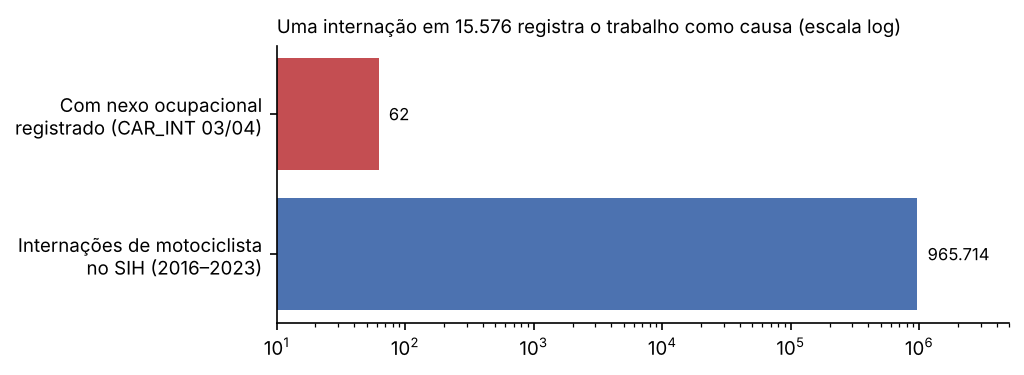
\includegraphics[width=0.85\textwidth,height=\textheight]{figuras/fig4_nexo.png}
\caption{Uma internação de motociclista em 15.576 registra o trabalho
como causa (SIH/SUS, 2016--2023).}
\end{figure}

A Previdência repete a cegueira. De 2019 a 2023 houve de 5 a 7
benefícios do INSS com CID V20--V29 por mil internações de motociclista
no SIH, e só 1 a 1,3 por mil com nexo acidentário reconhecido. Em
2024--2025 a razão salta para 12,5 e 15,4 por mil, mas a exploração
mostrou que se trata de \textbf{quebra de série}, não de mudança de
risco: a partir de nov/2023 a concessão por análise documental
(Atestmed) passa a dominar, e o atestado registra o código V muito mais
que a perícia (0,6--0,7 contra 0,03--0,13 por mil benefícios). Esse
canal responde por 65\% dos benefícios de motociclistas em 2024--2025;
anos dos dois lados da quebra não se comparam pelo total.

\hypertarget{precariedade-e-lucro}{%
\subsection{3.3 Precariedade e lucro}\label{precariedade-e-lucro}}

\textbf{Tabela 2 --- Motociclistas plataformizados (PNAD Contínua,
microdado; R\$ do 3T2025).}

\begin{longtable}[]{@{}llll@{}}
\toprule\noalign{}
& 2022 & 2024 & 2025 \\
\midrule\noalign{}
\endhead
\bottomrule\noalign{}
\endlastfoot
Pessoas (mil) & 211 & 351 & 405 \\
Informalidade & 77,6\% & 84,2\% & 85,2\% \\
Contribuem para a Previdência & 20,8\% & 21,6\% & 19,4\% \\
Horas por semana & 47,3 & 45,2 & 44,9 \\
Rendimento-hora real & R\$ 9,6 & R\$ 11,4 & R\$ 11,4 \\
Rendimento-hora real, setor privado & R\$ 16,6 & R\$ 17,7 & R\$ 18,4 \\
\end{longtable}

O pipeline reproduz, com erro de arredondamento, todos os números do
informativo do IBGE para 2024 (1.654 mil plataformizados; 71,1\%
informais; 35,9\% contribuintes; R\$ 15,4/h), o que valida o recorte
novo de motociclistas, que o IBGE não publica. Com 84\% de
informalidade, não há folha sobre a qual incida a contribuição de Riscos
Ambientais do Trabalho (RAT) que financia o benefício acidentário de
trabalhadores formais.

\begin{figure}
\centering
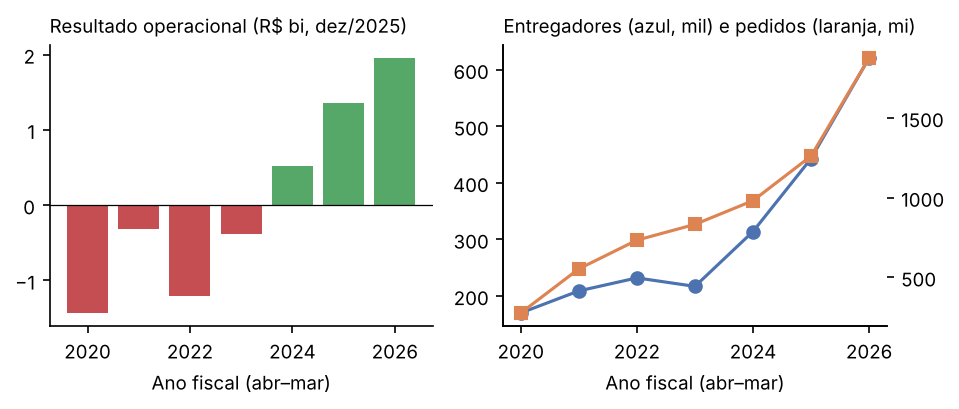
\includegraphics[width=1\textwidth,height=\textheight]{figuras/fig3_ifood.png}
\caption{iFood segundo as planilhas de KPI da Prosus: resultado
operacional em R\$ de dez/2025 (esq.) e entregadores ativos e pedidos
(dir.), por ano fiscal abril--março. A série de resultado emenda
\emph{trading profit} (até FY2024) e EBIT ajustado (a partir de
FY2025).}
\end{figure}

O resultado operacional do iFood cruza o zero em FY2024 e quase
quadruplica em dois anos; os entregadores ativos dobram de 314 mil para
621 mil (Figura 3). No ano civil de 2025 (interpolado), o EBIT ajustado
de R\$ 1,8 bilhão é cerca de \textbf{seis vezes} o que o SUS pagou com
todas as internações de motociclistas do país no mesmo ano (R\$ 288
milhões, ambos em R\$ de dez/2025). Com \textasciitilde1,7 bilhão de
pedidos no ano, menos de R\$ 0,20 por pedido cobriria essa conta. Esse
número dimensiona uma política, mas não a justifica: a fração das
internações atribuível à plataforma é exatamente o que a estimação
causal vai medir.

\hypertarget{o-tratamento-construuxeddo}{%
\subsection{3.4 O tratamento
construído}\label{o-tratamento-construuxeddo}}

\textbf{Tabela 3 --- Grupos do tratamento por faixa de população (Censo
2022) e taxa de disparo do placebo de 2016.}

\begin{longtable}[]{@{}
  >{\raggedright\arraybackslash}p{(\columnwidth - 10\tabcolsep) * \real{0.1667}}
  >{\raggedright\arraybackslash}p{(\columnwidth - 10\tabcolsep) * \real{0.1667}}
  >{\raggedright\arraybackslash}p{(\columnwidth - 10\tabcolsep) * \real{0.1667}}
  >{\raggedright\arraybackslash}p{(\columnwidth - 10\tabcolsep) * \real{0.1667}}
  >{\raggedright\arraybackslash}p{(\columnwidth - 10\tabcolsep) * \real{0.1667}}
  >{\raggedright\arraybackslash}p{(\columnwidth - 10\tabcolsep) * \real{0.1667}}@{}}
\toprule\noalign{}
\begin{minipage}[b]{\linewidth}\raggedright
Faixa
\end{minipage} & \begin{minipage}[b]{\linewidth}\raggedright
Municípios
\end{minipage} & \begin{minipage}[b]{\linewidth}\raggedright
\texttt{datado}
\end{minipage} & \begin{minipage}[b]{\linewidth}\raggedright
\texttt{sem\_quebra}
\end{minipage} & \begin{minipage}[b]{\linewidth}\raggedright
\texttt{coorte\_precoce}
\end{minipage} & \begin{minipage}[b]{\linewidth}\raggedright
Placebo 2016 dispara
\end{minipage} \\
\midrule\noalign{}
\endhead
\bottomrule\noalign{}
\endlastfoot
20--50 mil & 1.053 & 376 & 677 & --- & 0,7\% \\
50--100 mil & 338 & 264 & 74 & --- & 3,8\% \\
100--250 mil & 203 & --- & --- & 203 & 24,1\% \\
250 mil+ & 116 & --- & --- & 116 & 25,9\% \\
\textbf{Total} & \textbf{1.710} & \textbf{640} & \textbf{751} &
\textbf{319} & \\
\end{longtable}

A taxa de falso positivo do placebo define onde a regra vale. Abaixo de
100 mil habitantes ela é baixa (0,7\% e 3,8\%); acima, com muitas
aberturas, qualquer aceleração local passa no teste (≈ 25\%). Por isso
os 319 municípios de 100 mil+ --- todos com iFood já em 2019 --- formam
uma \textbf{coorte precoce} fora da estimação principal, e a variação
temporal vem dos 640 municípios \texttt{datado} de 20--100 mil.

\begin{figure}
\centering
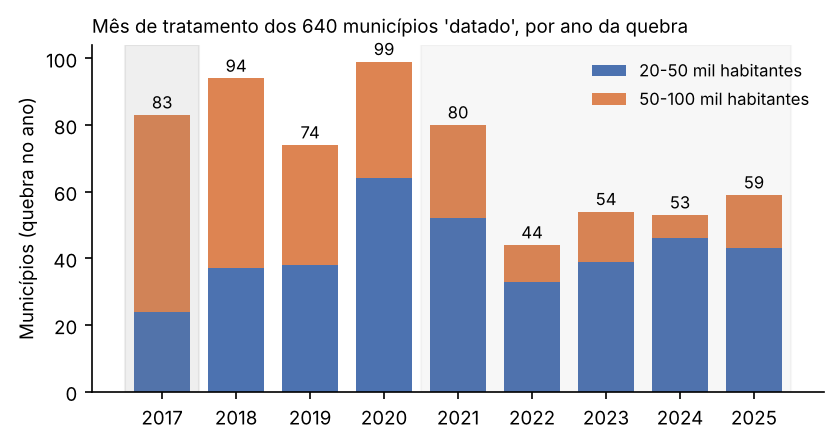
\includegraphics[width=0.95\textwidth,height=\textheight]{figuras/fig1_coortes.png}
\caption{Ano da quebra nos 640 municípios \texttt{datado}. Faixa cinza
escura: 2017, estrato de risco de quebra espúria (antes da frota própria
do iFood); cinza claro: 2021--2025, risco de contaminação pela entrega
de comércio eletrônico.}
\end{figure}

As quebras se espalham por todo o período (Figura 1), com pico em
2018--2021 --- coerente com o \emph{rollout} da frota própria do iFood
(cerca de 900 municípios em 2019 e 1.500 em 2023--2025). A Figura 2
mostra a adoção escalonada: ao fim de 2025, 46\% dos 1.391 municípios de
20--100 mil estão tratados, o que preserva um grupo
\emph{not-yet-treated} ao longo de toda a janela.

\begin{figure}
\centering
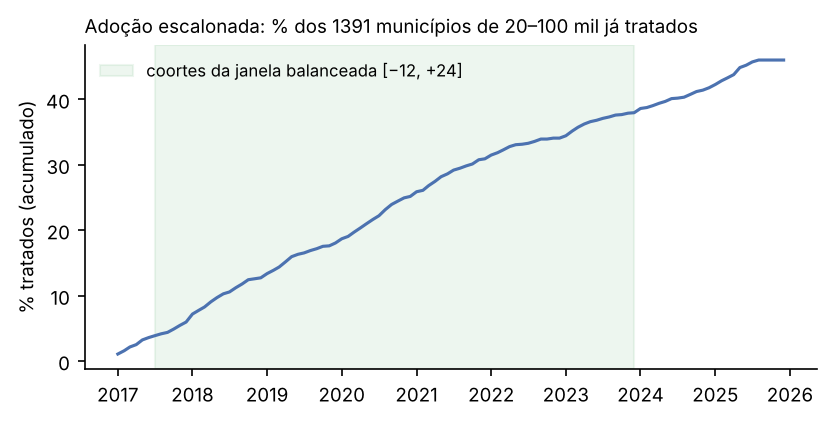
\includegraphics[width=0.95\textwidth,height=\textheight]{figuras/fig2_adocao_acumulada.png}
\caption{Proporção acumulada de municípios de 20--100 mil habitantes já
tratados. Em verde, as coortes que cabem na janela balanceada de
estimação.}
\end{figure}

\textbf{Janela de estimação.} Com a frota municipal começando em
jul/2016 e o SIH terminando em dez/2025, a janela balanceada {[}−12,
+24{]} admite coortes de 2017-07 a 2023-12: \textbf{478 dos 640}
municípios \texttt{datado}. Ficam de fora 50 com quebra anterior e 112
com quebra posterior, que voltam nas versões não balanceada e de
contagem.

\textbf{Tabela 4 --- Grupos por grande região.}

\begin{longtable}[]{@{}
  >{\raggedright\arraybackslash}p{(\columnwidth - 8\tabcolsep) * \real{0.2000}}
  >{\raggedright\arraybackslash}p{(\columnwidth - 8\tabcolsep) * \real{0.2000}}
  >{\raggedright\arraybackslash}p{(\columnwidth - 8\tabcolsep) * \real{0.2000}}
  >{\raggedright\arraybackslash}p{(\columnwidth - 8\tabcolsep) * \real{0.2000}}
  >{\raggedright\arraybackslash}p{(\columnwidth - 8\tabcolsep) * \real{0.2000}}@{}}
\toprule\noalign{}
\begin{minipage}[b]{\linewidth}\raggedright
Região
\end{minipage} & \begin{minipage}[b]{\linewidth}\raggedright
\texttt{datado}
\end{minipage} & \begin{minipage}[b]{\linewidth}\raggedright
\texttt{sem\_quebra}
\end{minipage} & \begin{minipage}[b]{\linewidth}\raggedright
\texttt{coorte\_precoce}
\end{minipage} & \begin{minipage}[b]{\linewidth}\raggedright
\% \texttt{datado} entre 20--100 mil
\end{minipage} \\
\midrule\noalign{}
\endhead
\bottomrule\noalign{}
\endlastfoot
Sudeste & 288 & 104 & 149 & 73\% \\
Sul & 168 & 48 & 55 & 78\% \\
Centro-Oeste & 54 & 45 & 25 & 55\% \\
Nordeste & 106 & 422 & 64 & 20\% \\
Norte & 24 & 132 & 26 & 15\% \\
\end{longtable}

A exploração revelou um desbalanço regional que não estava previsto: no
Nordeste e no Norte, só 15--20\% dos municípios de 20--100 mil têm
quebra, contra 73--78\% no Sul e no Sudeste. Isso pode refletir chegada
mais tardia das plataformas --- ou apenas menor propensão à formalização
via MEI, caso em que parte dos \texttt{sem\_quebra} nordestinos estaria
tratada sem ser vista. A seção 4 discute a consequência.

\hypertarget{discussuxe3o}{%
\section{4. Discussão}\label{discussuxe3o}}

\textbf{O que já se sabe.} A carga é grande (perto de 150 mil
internações por ano), crescente e invisível: o sistema de informação em
saúde vê o trabalho em uma internação a cada 15.576, e a Previdência, em
uma a duas por mil. A população exposta cresceu e se precarizou,
enquanto o setor tornou-se lucrativo. Esses fatos não dependem de
identificação causal e sustentam, por si, a política mais barata da
lista: tornar obrigatório o registro do nexo ``trabalho por plataforma''
na AIH e no SINAN.

\textbf{O que ainda não se sabe --- e por que esta versão não responde.}
Quanto do crescimento das internações é \emph{causado} pela chegada do
entregador por corrida. Essa fração é o que converte ``o SUS paga por
acidentes de moto'' em ``o SUS paga por acidentes que a remuneração por
corrida causou''. Optamos por não estimá-la antes do depósito do plano
no OSF: o número de escolhas defensáveis (agregação dos efeitos
dinâmicos, grupo de comparação, nível de cluster, janela, desfecho em
taxa ou contagem) é grande o bastante para que qualquer resultado obtido
antes do registro fosse suspeito de busca por especificação. O
estimando, o critério de inferência e as consequências de cada teste de
falha estão fixados.

\textbf{Limitações já conhecidas, com a direção do viés.} Três razões
fazem do coeficiente a ser estimado um \textbf{piso}, e são distintas:
(1) \emph{diluição} --- o desfecho inclui todos os motociclistas, não só
entregadores (desenho ecológico); (2) \emph{contaminação do pré-período}
--- o \emph{marketplace} já operava antes da frota própria; (3)
\emph{denominador endógeno} --- se a plataforma faz gente comprar moto,
a taxa é atenuada (teste 3). Além disso: o tratamento data a chegada de
\textbf{oferta de entregador formalizado}, de qualquer plataforma, não a
da plataforma X; quebras de 2017 podem ser espúrias e as de 2021+ podem
refletir a entrega de comércio eletrônico (ambas auditadas, com
consequência escrita); o município de residência não é o do acidente, o
que justifica o cluster regional; e o desbalanço regional da Tabela 4
sugere que \texttt{sem\_quebra} contém municípios tratados não
detectados, o que contamina o grupo de comparação e atenua o efeito. A
robustez pré-registrada que exclui os \texttt{sem\_quebra} responde
diretamente a isso; uma análise por região, exploratória e declarada
como tal, é o passo natural.

\textbf{Implicações.} O debate brasileiro é sobre vínculo; a
externalidade fiscal não depende dele. Se H1 for sustentada, a fração
atribuível dá a base de cálculo para uma contribuição acidentária das
plataformas sobre o valor das corridas --- equivalente funcional do RAT
---, ou um repasse por corrida ao SUS no molde do que o DPVAT fazia. Se
não for, a invisibilidade documentada aqui continua sendo, sozinha,
argumento para mudar o registro.

\hypertarget{conclusuxe3o}{%
\section{5. Conclusão}\label{conclusuxe3o}}

O trabalho responde ao primeiro objetivo --- medir carga, custo e
invisibilidade --- com números reproduzíveis e validados contra
referências externas: \textasciitilde150 mil internações de
motociclistas por ano no SUS, R\$ 288 milhões pagos em 2025, uma em
15.576 com nexo ocupacional registrado, numa força de trabalho 85\%
informal, ao lado de uma plataforma líder com R\$ 1,8 bilhão de
resultado operacional. Responde ao segundo objetivo construindo, sem
olhar o desfecho, um tratamento municipal datado para 640 municípios,
com hiperparâmetros calibrados contra placebo e validação externa e com
taxa de falso positivo baixa onde é usado. O terceiro objetivo está
especificado e travado em pré-registro; a estimação causal e a auditoria
cega do tratamento são as próximas etapas.

\hypertarget{materiais-complementares}{%
\section{Materiais complementares}\label{materiais-complementares}}

\begin{itemize}
\tightlist
\item
  \textbf{Código e documentação:} \texttt{github.com/mrcsvg/vcemal}
  (MIT; textos CC BY 4.0). Pipeline completo por \texttt{Makefile};
  \texttt{make\ test} roda sem rede e sem dado. Log de 43 decisões
  datadas em \texttt{docs/decisoes.md}; dicionário do painel em
  \texttt{docs/dicionario-painel.md}.
\item
  \textbf{Dados:} não versionados, por volume (D-009); todas as fontes
  são públicas e o inventário
  (\texttt{docs/anexo-a-inventario-fontes-de-dados.md}) traz órgão, URL,
  cobertura, formato e latência de cada uma. Versionados: tratamento
  congelado (com hash) e transcrição citada da Prosus.
\item
  \textbf{Script desta versão:} \texttt{artigo/analise\_artigo.py} gera
  as Figuras 1--4 e as tabelas de \texttt{artigo/tabelas/} a partir só
  dos arquivos versionados, sem rede.
\item
  \textbf{Bibliotecas:} Python ≥ 3.11; pandas, numpy, pyarrow, PySUS ≥
  2.11, matplotlib, requests (versões em \texttt{pyproject.toml}).
\item
  \textbf{Hiperparâmetros:} regra de quebra \emph{k} = 2, \emph{N} = 5,
  α = 0,01, linha de base de 24 meses, janela de 6 meses, piso de 0,5
  abertura; grade avaliada \emph{k} ∈ \{1,5; 2; 3\} × \emph{N} ∈ \{3; 5;
  8\}. Estimação: janela {[}−12, +24{]}, comparação
  \emph{not-yet-treated}, cluster em região imediata, α = 0,05
  bilateral. Semente da auditoria: 20261011.
\item
  \textbf{Pré-registro:} OSF \textbf{{[}DOI/URL{]}}; texto do formulário
  em \texttt{docs/pre-registro/deposito-osf.md}.
\item
  \textbf{Checklist REFORMS:} documento anexo
  (\texttt{artigo/reforms.md}).
\end{itemize}

\hypertarget{declarauxe7uxe3o-de-uso-de-ia-generativa}{%
\section{Declaração de uso de IA
generativa}\label{declarauxe7uxe3o-de-uso-de-ia-generativa}}

A equipe utilizou o assistente Claude (Anthropic), via Claude Code, como
apoio à elaboração e revisão de código do pipeline e de testes, à
organização do log de decisões e à redação e revisão textual desta
versão do artigo e do checklist REFORMS. Todas as decisões
metodológicas, os números reportados e as referências foram conferidos
pela equipe, que assume integral responsabilidade pelo conteúdo.
\textbf{{[}AJUSTAR CONFORME O USO EFETIVO DA EQUIPE{]}}

\hypertarget{referuxeancias}{%
\section{Referências}\label{referuxeancias}}

ABRAMET --- Associação Brasileira de Medicina de Tráfego. Internações de
motociclistas no SUS (tabulação do SIH/SUS), 2024.

CALLAWAY, B.; SANT'ANNA, P. H. C. Difference-in-differences with
multiple time periods. \emph{Journal of Econometrics}, v. 225, n.~2,
p.~200--230, 2021.

CARVALHO, C. H. R. \emph{Custos dos acidentes de trânsito no Brasil:
estimativa simplificada com base na atualização das pesquisas do Ipea
sobre custos de acidentes nos aglomerados urbanos e rodovias}. Texto
para Discussão n.~2565. Brasília: Ipea, 2020.

DATASUS. \emph{Sistema de Informações Hospitalares do SUS (SIH/SUS) ---
Estrutura dos arquivos RD e notas técnicas de morbidade hospitalar por
causas externas}. Brasília: Ministério da Saúde.

GOODMAN-BACON, A. Difference-in-differences with variation in treatment
timing. \emph{Journal of Econometrics}, v. 225, n.~2, p.~254--277, 2021.

IBGE. \emph{PNAD Contínua: Teletrabalho e trabalho por meio de
plataformas digitais 2024}. Rio de Janeiro: IBGE, 2025.

KAPOOR, S. et al.~REFORMS: Consensus-based recommendations for
machine-learning-based science. \emph{Science Advances}, v. 10, n.~18,
eadk3452, 2024.

NOSEK, B. A. et al.~The preregistration revolution. \emph{Proceedings of
the National Academy of Sciences}, v. 115, n.~11, p.~2600--2606, 2018.

PROSUS N.V. \emph{KPI datasheets}, anos fiscais 2021 a 2026. Amsterdã:
Prosus. Disponível em: prosus.com (URLs por célula em
\texttt{docs/fontes/ifood\_prosus.csv}).

ROTH, J. et al.~What's trending in difference-in-differences? A
synthesis of the recent econometrics literature. \emph{Journal of
Econometrics}, v. 235, n.~2, p.~2218--2244, 2023.

SUN, L.; ABRAHAM, S. Estimating dynamic treatment effects in event
studies with heterogeneous treatment effects. \emph{Journal of
Econometrics}, v. 225, n.~2, p.~175--199, 2021.

\end{document}
